\newcommand{\cvsID}{$ $Id: simsetup.tex,v 1.2 2006/11/13 14:57:41 ali Exp $ (CVS)$}
\documentclass{article}
\usepackage{graphicx}
\usepackage{natbib}
\usepackage{graphicx}
\bibliographystyle{plainnat}
\usepackage{fancyheadings}
\usepackage{tabularx}
\usepackage{alltt, parskip, boxedminipage}
\usepackage{makeidx, multirow, longtable, tocbibind, amssymb}
%\usepackage{fullpage}
\makeindex
\usepackage[usenames]{color}
\definecolor{darkblue}{rgb}{0,0.05,0.35}

\usepackage[dvips, pagebackref, pdftitle={}, pdfcreator={epydoc 2.1}, bookmarks=true, bookmarksopen=false, pdfpagemode=UseOutlines, colorlinks=true, linkcolor=black, anchorcolor=black, citecolor=black, filecolor=black, menucolor=black, pagecolor=black, urlcolor=darkblue]{hyperref}
\setlength{\textheight}{21.5cm}
\setlength{\textwidth}{18cm}
\setlength{\hoffset}{-3.0cm}
\setlength{\footskip}{1.5cm}
\setlength{\headsep}{2.5cm}
\setlength{\voffset}{-2.5cm}
\newlength{\BCL} % base class length, for base trees.

\usepackage{everyshi}
 \makeatletter
 \let\totalpages\relax
 \newcounter{mypage}
 \EveryShipout{\stepcounter{mypage}}
 \AtEndDocument{\clearpage
    \immediate\write\@auxout{%
     \string\gdef\string\totalpages{\themypage}}}
 \makeatother

\newcommand{\daspfooter}{

\includegraphics[height=1cm]{durlogo.eps}
{\bf \large Centre for \AA dvanced Instrumentation}
}
\newcommand{\daspheaderl}{

\includegraphics[height=1cm]{durlogo.eps}
\begin{tabularx}{9cm}{c}
\Large {\bf \dasptitle} \\ \large {\bf(\daspdoctype)}\\
\rightmark\hspace{0.1cm}
\end{tabularx}
\vfill
}
\newcommand{\daspheaderc}{
}
\newcommand{\daspheaderr}{
\begin{tabular}{|l|l|}\hline
Doc. number: & \daspdocno \\ \hline
Release date: & \daspreleasedate \\ \hline
Issue number: & \daspissue \\ \hline
Page number: & Page \thepage \ of \totalpages \\ \hline
Author(s) & \daspauthorname \\ \hline
\end{tabular}


}

\pagestyle{fancy}
\cfoot[]{}
\lfoot[\daspfooter]{\daspfooter}
\lhead[\daspheaderl]{\daspheaderl}
\chead[\daspheaderc]{\daspheaderc}
\rhead[\daspheaderr]{\daspheaderr}
\renewcommand{\sectionmark}[1]{\markboth{#1}{#1}}

\newenvironment{Ventry}[1]%
  {\begin{list}{}{%
    \renewcommand{\makelabel}[1]{\texttt{##1:}\hfil}%
    \settowidth{\labelwidth}{\texttt{#1:}}%
    \setlength{\leftmargin}{\labelsep}%
    \addtolength{\leftmargin}{\labelwidth}}}%
  {\end{list}}


\begin{document}
\newcommand{\esoproject}{AO Simulation Project}
\newcommand{\esotitle}{AO Simulation creation}
\newcommand{\esodocno}{AOSIM-SET-UoD-001}
\newcommand{\esodoctype}{Internal}
\newcommand{\esoissue}{0.1.1}
\newcommand{\esoreleasedate}{\today}
\newcommand{\esoauthorname}{Alastair Basden}
\newcommand{\esoauthortype}{AO sim team member}
\newcommand{\esoapprovername}{Alastair Basden}
\newcommand{\esoapprovertype}{AO sim team member}
\newcommand{\esoreleasername}{Alastair Basden}
\newcommand{\esoreleasertype}{AO sim team member}
\newcommand{\esoreviewername}{Alastair Basden}
\newcommand{\esoreviewertype}{AO sim team member}
\newcommand{\esochangerecord}{
\begin{tabular}{|l|l|l|l|}
\hline
Issue number & Release date & section(s) affected & Description of
change/remarks\\ \hline
0.1.0 & 051111 & All & First draft \\ \hline
0.1.1 & 051111 & All & Corrections made to first draft\\ \hline
\end{tabular}
}
\newcommand{\esonotificationlist}{
Alastair Basden\\
Francois Assemat\\
Richard Wilson\\
Tim Morris\\
Tim Butterley\\
}
\newcommand{\esoabbreviations}{
\begin{tabular}{rl}
AO & Adaptive Optics\\
ESO & European Southern Observatory\\
\end{tabular}
}
\newcommand{\esoapplicabledocs}{
\begin{tabular}{|l|l|l|}\hline
AD Number & Document title & Doc number/publication/location \\ \hline
AD01 & Simulation API document & AOSIM-API-UoD-001\\ \hline
AD02 & Simulation for dummies document & AOSIM-DUM-UoD-001\\ \hline
\end{tabular}
}
\newcommand{\esorefdocs}{
\begin{tabular}{|l|l|l|}\hline
RD number & Document title & Doc number/publication/location \\ \hline
RD01 & Durham FPGA website & www.durham.ac.uk/rtcs.project \\ \hline
\end{tabular}
}
\title{\esotitle}



\thispagestyle{empty}
%This next command provides the CVS tag.  If you want a cvs tag on
%your document, add the following line at the start of the document,
%after replacing the & signs with dollar signs...
%\newcommand{\cvsID}{& &Id& (CVS)&}
\providecommand{\cvsID}{CVS ID not provided: document made on \today}

\begin{center}

\includegraphics{durlogo.eps}
\end{center}
\vspace{0.5cm}
\Huge
\begin{center}
\daspproject\\
\end{center}
\Large
\vspace{1cm}


{\bf 
\begin{tabular}{ll}
Document title: & \dasptitle \vspace{0.5cm}\\ 

Documentation number: & \daspdocno \vspace{0.5cm}\\ 

Document type: & \daspdoctype \vspace{0.5cm}\\ 

Issue number:& \daspissue \vspace{0.5cm}\\ 

Release date: & \daspreleasedate \\ 

\end{tabular}
}

\normalsize
\vfill

\begin{tabular}{|l|l|l|p{5cm}|}
\hline
Document & \daspauthorname & Signature &\\
prepared by & \daspauthortype & and date &\\ \hline
Document & \daspapprovername & Signature &\\
approved by & \daspapprovertype & and date &\\ \hline
Document & \daspreleasername & Signature &\\
released by & \daspreleasertype & and date &\\ \hline
Document & \daspreviewername & Signature &\\
reviewed by & \daspreviewertype & and date &\\ \hline
\end{tabular}

\small
%\begin{alltt}
\cvsID
%\end{alltt}
\normalsize
%\lfoot[\daspfooter]{\daspfooter}
%\lhead[\daspheaderl]{\daspheaderl}
%\chead[\daspheaderc]{\daspheaderc}
%\rhead[\daspheaderr]{\daspheaderr}
%\renewcommand{\sectionmark}[1]{\markboth{#1}{#1}}

\pagebreak
a
\vspace{2cm}
\begin{center}
\Large
{\bf Change record\\ \vspace{1cm}}
\normalsize
\daspchangerecord
\end{center}
\vspace{2cm}

\begin{center}
\Large
{\bf Notification list\\ \vspace{1cm}}
\normalsize
\daspnotificationlist
\end{center}

\pagebreak

\begin{center}
\Large
{\bf Acronyms and abbreviations\\ \vspace{1cm}}
\normalsize
\daspabbreviations
\end{center}

\pagebreak

\begin{center}
\Large
{\bf Applicable documents\\ \vspace{1cm}}
\normalsize

\daspapplicabledocs
\end{center}
\vspace{2cm}

\begin{center}
\Large
{\bf Reference documents \\ \vspace{1cm}}
\normalsize

\dasprefdocs
\end{center}

\pagebreak
\tableofcontents
\pagebreak

\section{Introduction}
This guide is intended to provide information about the simulation
setup GUI (simsetup.py), part of the AO simulation package.  Further
information about the AO simulation package can be found in
\citet{overview}.

The simulation setup GUI is used to create a simulation by linking
together the various modules that are required, and specifying which
processor (in a multi-processor system) they should run on.  Setting
up a large simulation by hand is a laborious task which can take
several days.  By using the setup GUI, this time can be reduced to
minutes and a few mouse clicks.  Additionally, it is then trivial to
optimise the simulation performance by re-balancing the processes,
placing different modules on different computing nodes.  Previously,
this was time consuming.

The setup GUI does not include simulation parameter definition.  This
should be carried out using the parameter GUI \citep{simparamgui} once
the simulation has been set up.  At the time of writing, the
interaction between the setup and parameter GUIs is minimal.  However,
should further effort become available, it would be possible to
interlink these two pieces of software.


\section{The simsetup GUI}
Fig.~\ref{fig:simsetup} shows the simulation setup GUI during use.
The functionality of this GUI will now be described.
\begin{figure}
\begin{tabular}{ll}
\includegraphics[width=4cm]{pics/simsetuptoolbar.eps} &
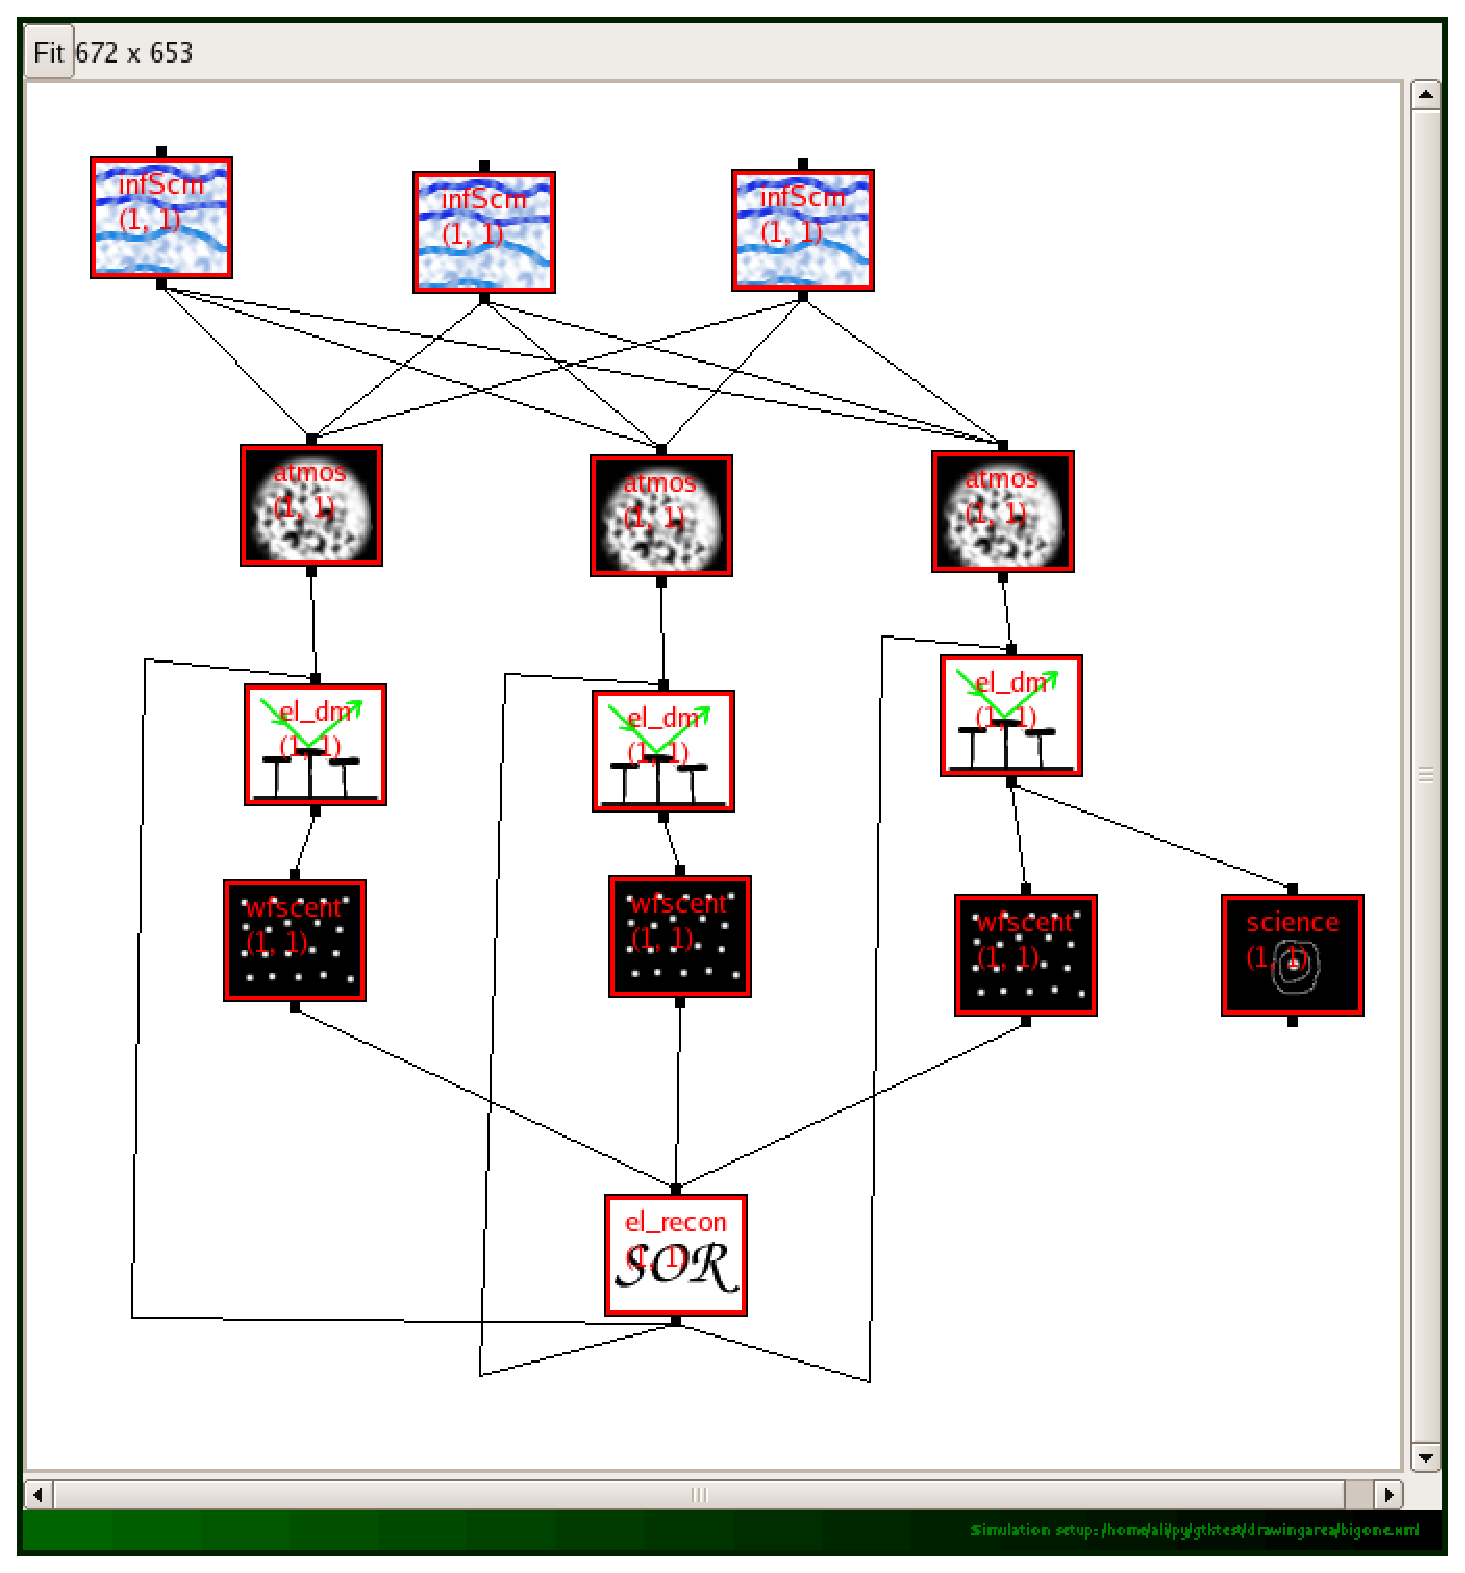
\includegraphics[width=12cm]{pics/simsetupmain.eps} \\
\end{tabular}
\caption{A screenshot of the simulation setup GUI during use showing
the toolbar on the left and the workspace window on the right.}
\label{fig:simsetup}
\end{figure}

As shown in Fig.~\ref{fig:simsetup}, the simulation setup GUI consists
of two windows.  The first of these is the toolbar window, which
provides the user with the various different tools that can be used to
create a simulation.  The second window is the workspace window where
the simulation is set up, by placing different modules, and linking
them together.

\subsection{The toolbar window}
The toolbar window is used to select the operation you wish to perform
(e.g.\ placing a new module, connecting modules together etc.), and to
set preferences associated with modules and connections.  The menu bar
for this window contains standard ``open'', ``save'', ``save as'',
``new'' and ``exit'' entries.  The preferences menu also contains an
entry to reload the science widgets.  When selected, the user will be
prompted for a filename, and this file will be used to place entries
in the node pane and the module selection pane of the toolbar window
(these panes are immediately below the six buttons, and above the
object preferences pane).  It is unlikely a user will need to use this
option unless they wish to add their own modules to the simulation,
which are not in CVS.  

The preferences menu also contains a ``connect to paramgui'' entry,
which when selected will present you with an entry box for the
paramgui that you wish to connect to (this must be running).  Here,
you can enter the hostname (optional) and the port on which this
paramgui is listening.  The default port is 8990, and the actual port
used is displayed towards the bottom of the paramgui window.  If you
are running paramgui and simsetup on the same computer, you do not
need to give a hostname.  Once connected, you can disconned simply be
selecting this menu option again.  When connected, the paramgui will
be told to display parameters for the currently selected simulation
module in the simsetup main window.  If the paramgui does not
currently hold information about these parameters, they will be
created for you.

Currently none of the other menu entries are functional.  

\subsubsection{Button selections}
Below this menubar are six buttons used for creation of the
simulation.  ``Select'' puts the user in select mode, allowing them to
select and move objects in the workspace window, and set their
preferences.  The ``New module'' button allows the user to place new
modules of the type currently selected in the module selection pane
(in the Figure, the infinite phasescreen module is currently
selected).  When the user then clicks in the workspace window, a new
module will be placed into the simulation.  The ``Connect'' button
allows the user to connect the inputs and outputs of modules together.
This is done by clicking on a module, and clicking on the module to
which it should connect.  Clicks in a blank part of the workspace will
add a point to the connecting line, anchoring the line at this point
on the workspace.  However, a line can only begin and end on a module.
By default, connections go from the parent module to the child module.
However, by clicking on the input of a module when initiating a
connection, the reverse can be made to happen, ie this module is then
the child.  The ``Delete'' button allows the user to click on a module
or connection line in the workspace window to remove this item.  The
``Re-place'' button allows the user to change the processing node on
which the module will run.  The current node is shown in the node
selection pane (in this case, node 1), and any modules that are then
clicked on (when ``Re-place'' is selected) will be placed on this
node.  When new modules are created, they will be placed on the node
which is currently selected.  The modules in the workspace window are
colour coded such that the outside of the module matches the colour of
the node with which it is associated.  The ``Generate'' button is used
to generate Python code for the simulation.  The user will be prompted
for a filename.  The generated Python code can then be run once a
parameter file exists for it.

These button selections have keyboard shortcuts when used in the main
window, namely, the first letter of the button (e.g.\ ``n'' to go into
``new module'' mode).

\subsubsection{The node and module selection panes}
Below the buttons are the node pane and module selection pane, which
have been discussed above.  

\subsubsection{The object preferences pane}
The object preferences pane is below the module selection pane.
This pane can be made to disappear by clicking on the object
preferences title.  When an object is selected in the workspace
window, its preferences can be set here.  The name is optional, and if
given will be used in the Python code as the name of the object, for
example, you may wish to call a phase screen at 2km a PhaseScrn2000m
object.  If no name is given, the object will be appended to a list.
It is unlikely that you will bother setting these names.  

The CPU preference determines the node and CPU number on which this
process will run, and can be changed by typing, or by clicking on the
object in the workspace window when the ``Re-place'' button is
selected.  The CPU is a tuple of processing node, CPU number.  On the
Cray XD1, the major (first) number will range from 1--6 (6 nodes), and
the minor (second) number will range from 1--2 (2 CPUs per node).
Objects with the same major number but a different minor number will
run in separate processes, using shared memory to communicate.
Objects with a different major number will run on different nodes,
using MPI to communicate.  Objects with the same major and minor
number will run in the same process.

The feedback preference should be selected for objects that provide
feedback, for example a reconstructor.  

The args text entry is to allow the user to specify optional arguments
to be used when the selected object is created by the Python
interpreter when the simulation is run.  Typically, you will only want
to set the ID string, which is used to give the module a unique name
when searching the parameter file for parameters.  This can be set
simply by typing the name in the entry, for example ``2000m'' for a
phasescreen at 2000m, and ``0m'' for a phasescreen at 0m (the
parameter file would then contain modules for infScrn\_2000m and
infScrn\_0m).  If other options are needed, they can be set as a
dictionary, for example ``{'myoption':1,'idstr':'2000m'}''.  

The two text entries below this are for code to run immediately before
and after the object is created.  It is unlikely that you will need to
add anything here, though they are there just in case, to provide
extra functionality.  

When a connection line is selected in the workspace window, only the
name of the line can be set.  This name is then the name that is
passed to the object receiving the data from this connection, and is
optional.  In most cases you do not (should not) set a name.  However,
a deformable mirror object requires a connection with a name ``atmos''
and a connection with a name ``recon''.  An infAtmos module requires
names equal to the ID string of the infScrn from which they are
connected.  

\subsubsection{The Initialisation text pane}
The initialisation text pane (which can be made to vanish by clicking
on the initialisation text) is used to insert code which should be run
after simulation modules have been imported, but before any objects
are created (except for the control object).  This can provide
optional functionality.

\subsubsection{The Finalisation text pane}
The finalisation text pane (which can be made to vanish by clicking on
the finalisation text) is used to insert code to be run after the
simulation has ended, for example to save data, or tidy up the
simulation.  This can provide optional functionality.

\subsection{The workspace window}
The workspace window contains a canvas where simulation objects are
placed, moved around and connected together.  Fig.~\ref{fig:simsetup}
shows a simulation being set up, with three atmospheric phase screens,
each of which is connected to a atmospheric pupil phase module (one
for one of three directions).  The system then contains a deformable
mirror (shown by three objects here, one for each viewing direction),
three wavefront sensors (one for each viewing direction), and a
reconstructor, which takes data from each wavefront sensor, and then
passes instructions back to the deformable mirror module.  There is
also a science module, which is viewing a target in the third
direction.  It is important to note that although we are only
simulating one telescope, and one deformable mirror here, three
atmospheric pupil phase objects and three deformable mirror objects
are required, as we treat different source directions as different
objects (this allows better parallelisation of the simulation).

Each object in the workspace window has an outer frame coloured
dependent on the node on which it is placed, a graphic allowing quick
visual determination of the object, and some identifying text on three
lines, containing the type of object, the node on which it is run, and
the optional ID string.  The output of an object is shown by the small
black box at the bottom of the object, and the input by the small
black box at the top.  Data passes from the output of one module to
the input of the next.

\subsubsection{The Fit button}
The ``Fit'' button at the top left hand corner of the workspace window
can be used to minimise the space taken up by the simulation.  Press
it, and you will see what I mean -- nothing really spectacular, just
shifts the whole simulation about.

\section{Setup XML file}
When a simsetup project is saved, an XML file is created.  This can be
edited by hand if necessary (though with care!).  Eventually, it will
be possible to place the setup xml, the parameter xml and the simctrl
xml all within the same XML file, and then a command ``aosim'' can be
used on this file to create and run the simulation, and display the
control GUI.  This is not yet functioning.

\section{Python executable}
When the generate button is pressed, a Python executable will be
created.  The top line of this file will be a comment suggesting how
the simulation should be run (giving the form of the MPI command).
You do not have to follow this suggestion, for example, you can run on
other nodes instead.  However, you should take care when doing this.
It is just possible that the algorithm used to determine the order in
which objects are executed on each node is not perfect.  If this is
the case, you may find the simulation freezes during the first
iteration of the simulation.  If this happens, please let AGB know.
You can always try re-jigging the execOrder list.  Such freezing has
not occured to AGB yet, but has not yet undergone extensive testing.  

\section{Checklist}
There are a number of things that should be checked when setting up a
simulation.  
\begin{enumerate}
\item All objects have been placed in the workspace window.
\item All connections have been made.
\item The preferences for objects (i.e.\ the ID string in the args
text entry) have been set if necessary, to identify different objects.
\item The name (a preference) of connection lines has been set where
needed, which typically is for lines connecting to an infAtmos module,
and to a deformable mirror module.
\item The objects have been allocated to different nodes as required.
\item Any finalisation text has been added.
\item The project has been saved.
\end{enumerate}

\section{XML file format}
The simsetup GUI saves the user document in XML file format.  This has
the standard aosim tag, and within this is a simSetup tag.  Within
this tag there are then simulationObject tags.  Each of these tags has
attributes named cpu, import, object, pos, tag, shortname, pixmap,
feedback, pyname, args, connectto, connectfrom and textcol.  Unless
you are a developer of the GUI, you will not need to know this
information.  Within the simulationObject tag, there are tags for
lines, endlines, parentNames, precode and postcode.  Within the
simSetup tag there are also optional precode and postcode tags.


\section{Conclusion}
The simulation setup GUI has been described, and you should now be
able to use it to set up small and large simulations.

\section{Work to do}
There are a number of things that could do with improvement in the
simulation setup GUI.  These have not yet been determined.

That should keep someone busy for a couple of weeks anyway!
\bibliography{references}
\printindex
\end{document}
